\documentclass[fleqn]{article}
\usepackage[margin=1in]{geometry}
\usepackage[nodisplayskipstretch]{setspace}
\usepackage{amsmath, nccmath, bm}
\usepackage{amssymb}
\usepackage{enumitem}
\usepackage{graphicx}
\usepackage{float}
\usepackage{xcolor}
\usepackage{listings}

\newcommand{\zerodisplayskip}{
	\setlength{\abovedisplayskip}{0pt}%
	\setlength{\belowdisplayskip}{0pt}%
	\setlength{\abovedisplayshortskip}{0pt}%
	\setlength{\belowdisplayshortskip}{0pt}%
	\setlength{\mathindent}{0pt}}
	

\definecolor{vgreen}{RGB}{104,180,104}
\definecolor{vblue}{RGB}{49,49,255}
\definecolor{vorange}{RGB}{255,143,102}

\lstdefinestyle{verilog-style}
{
    language=Verilog,
    basicstyle=\small\ttfamily,
    keywordstyle=\color{vblue},
    identifierstyle=\color{black},
    commentstyle=\color{vgreen},
    numbers=left,
    numberstyle=\tiny\color{black},
    numbersep=10pt,
    tabsize=8,
    moredelim=*[s][\colorIndex]{[}{]},
    literate=*{:}{:}1
}

\makeatletter
\newcommand*\@lbracket{[}
\newcommand*\@rbracket{]}
\newcommand*\@colon{:}
\newcommand*\colorIndex{%
    \edef\@temp{\the\lst@token}%
    \ifx\@temp\@lbracket \color{black}%
    \else\ifx\@temp\@rbracket \color{black}%
    \else\ifx\@temp\@colon \color{black}%
    \else \color{vorange}%
    \fi\fi\fi
}
\makeatother

\title{Homework 1}
\author{Owen Sowatzke}
\date{February 9, 2025}

\begin{document}

	\offinterlineskip
	\setlength{\lineskip}{12pt}
	\zerodisplayskip
	\maketitle
	
	\begin{enumerate}
		\item Given below is an illustrative layout of an inverter. Write down the material layer used according to color and arrange them in the order of fabrication.
		
		\begin{figure}[H]				
			\centerline{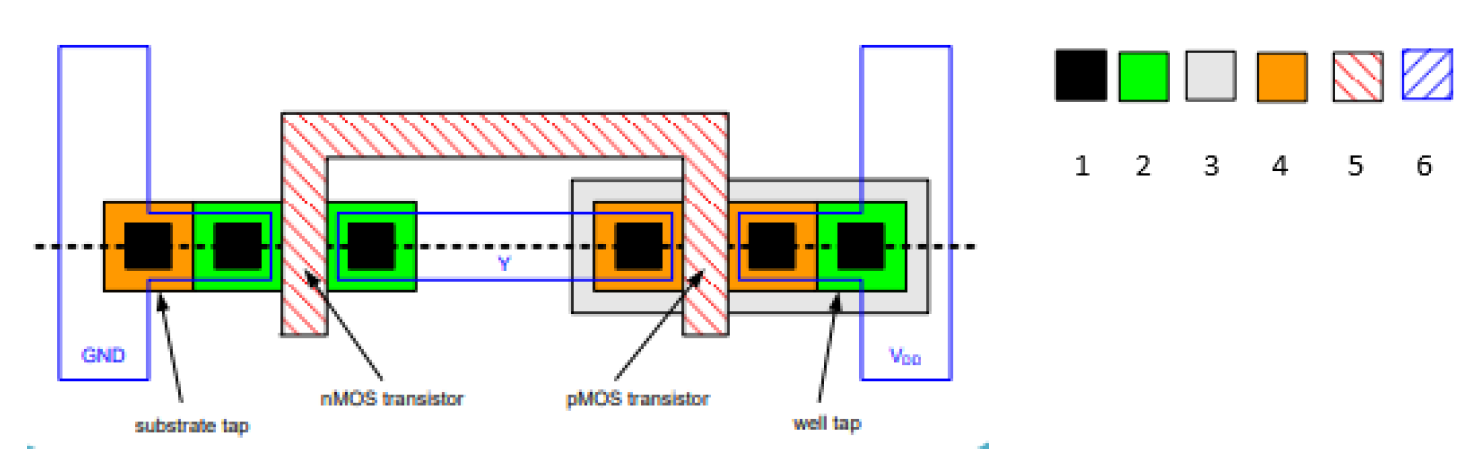
\includegraphics[width=0.8\textwidth]{inverter_layout.png}}
			\label{fig::inverter_layout}
		\end{figure}
		
		The materials in the layout are defined as follows:
		
		\begin{itemize}
			\item Material 1 (solid black) is contact material. It is made of metal (usually aluminum).
			\item Material 2 (solid green) is n+ diffusion (heavily doped n-type semiconductor [usually Si])
			\item Material 3 (solid gray) is the n-well (lightly doped n-type semiconductor [usually Si])
			\item Material 4 (solid orange) is the p+ diffusion (heavily doped p-type semiconductor [usually Si])
			\item Material 5 (striped red) is the polysilicon.
			\item Material 6 (striped blue) is the metal1 (usually aluminum)
		\end{itemize}
		
		The material layers are fabricated from the bottom up in the following order:
		
		\begin{enumerate}
			\item[1.] Material 3 (the n-well)
			\item[2.] Material 5 (polysilicon)
			\item[3.] Material 2 (n+ diffusion)
			\item[4.] Material 3 (p+ diffusion)
			\item[5.] Material 1 (contact)
			\item[6.] Material 6 (metal1)
		\end{enumerate}
		
		\item Illustrate the CMOS Layout and Stick diagram for the following Boolean expressions.
		
		\begin{enumerate}
			\item $Y = (A+B)\cdot(C+D)$
			
			In CMOS circuit design, we implement circuits that are the complement of boolean expressions. Because the provided expression is not in complement form, we must design a circuit to get $\bar{Y}$ and append an inverter to get $Y$.
			
			We start by designing the pull-down circuit to get $\bar{Y}$. We replace each "or" with a parallel set of nmos gates and each "and" with a series of nmos gates. The pull-down circuit is shown in the bottom half of Figure \ref{fig::cmos_layout_problem_2a}. We can then use the rule of conduction complements to design the pull-up circuit. To do so, we replace each parallel set of nmos gates with a series of pmos gates and each series of nmos gates with a parallel set of nmos gates. The resulting pull-up circuit is shown in the top half of Figure \ref{fig::cmos_layout_problem_2a}. The output $\bar{Y}$ is then fed into an inverter to get $Y$.
			
			\begin{figure}[H]
				\centerline{\fbox{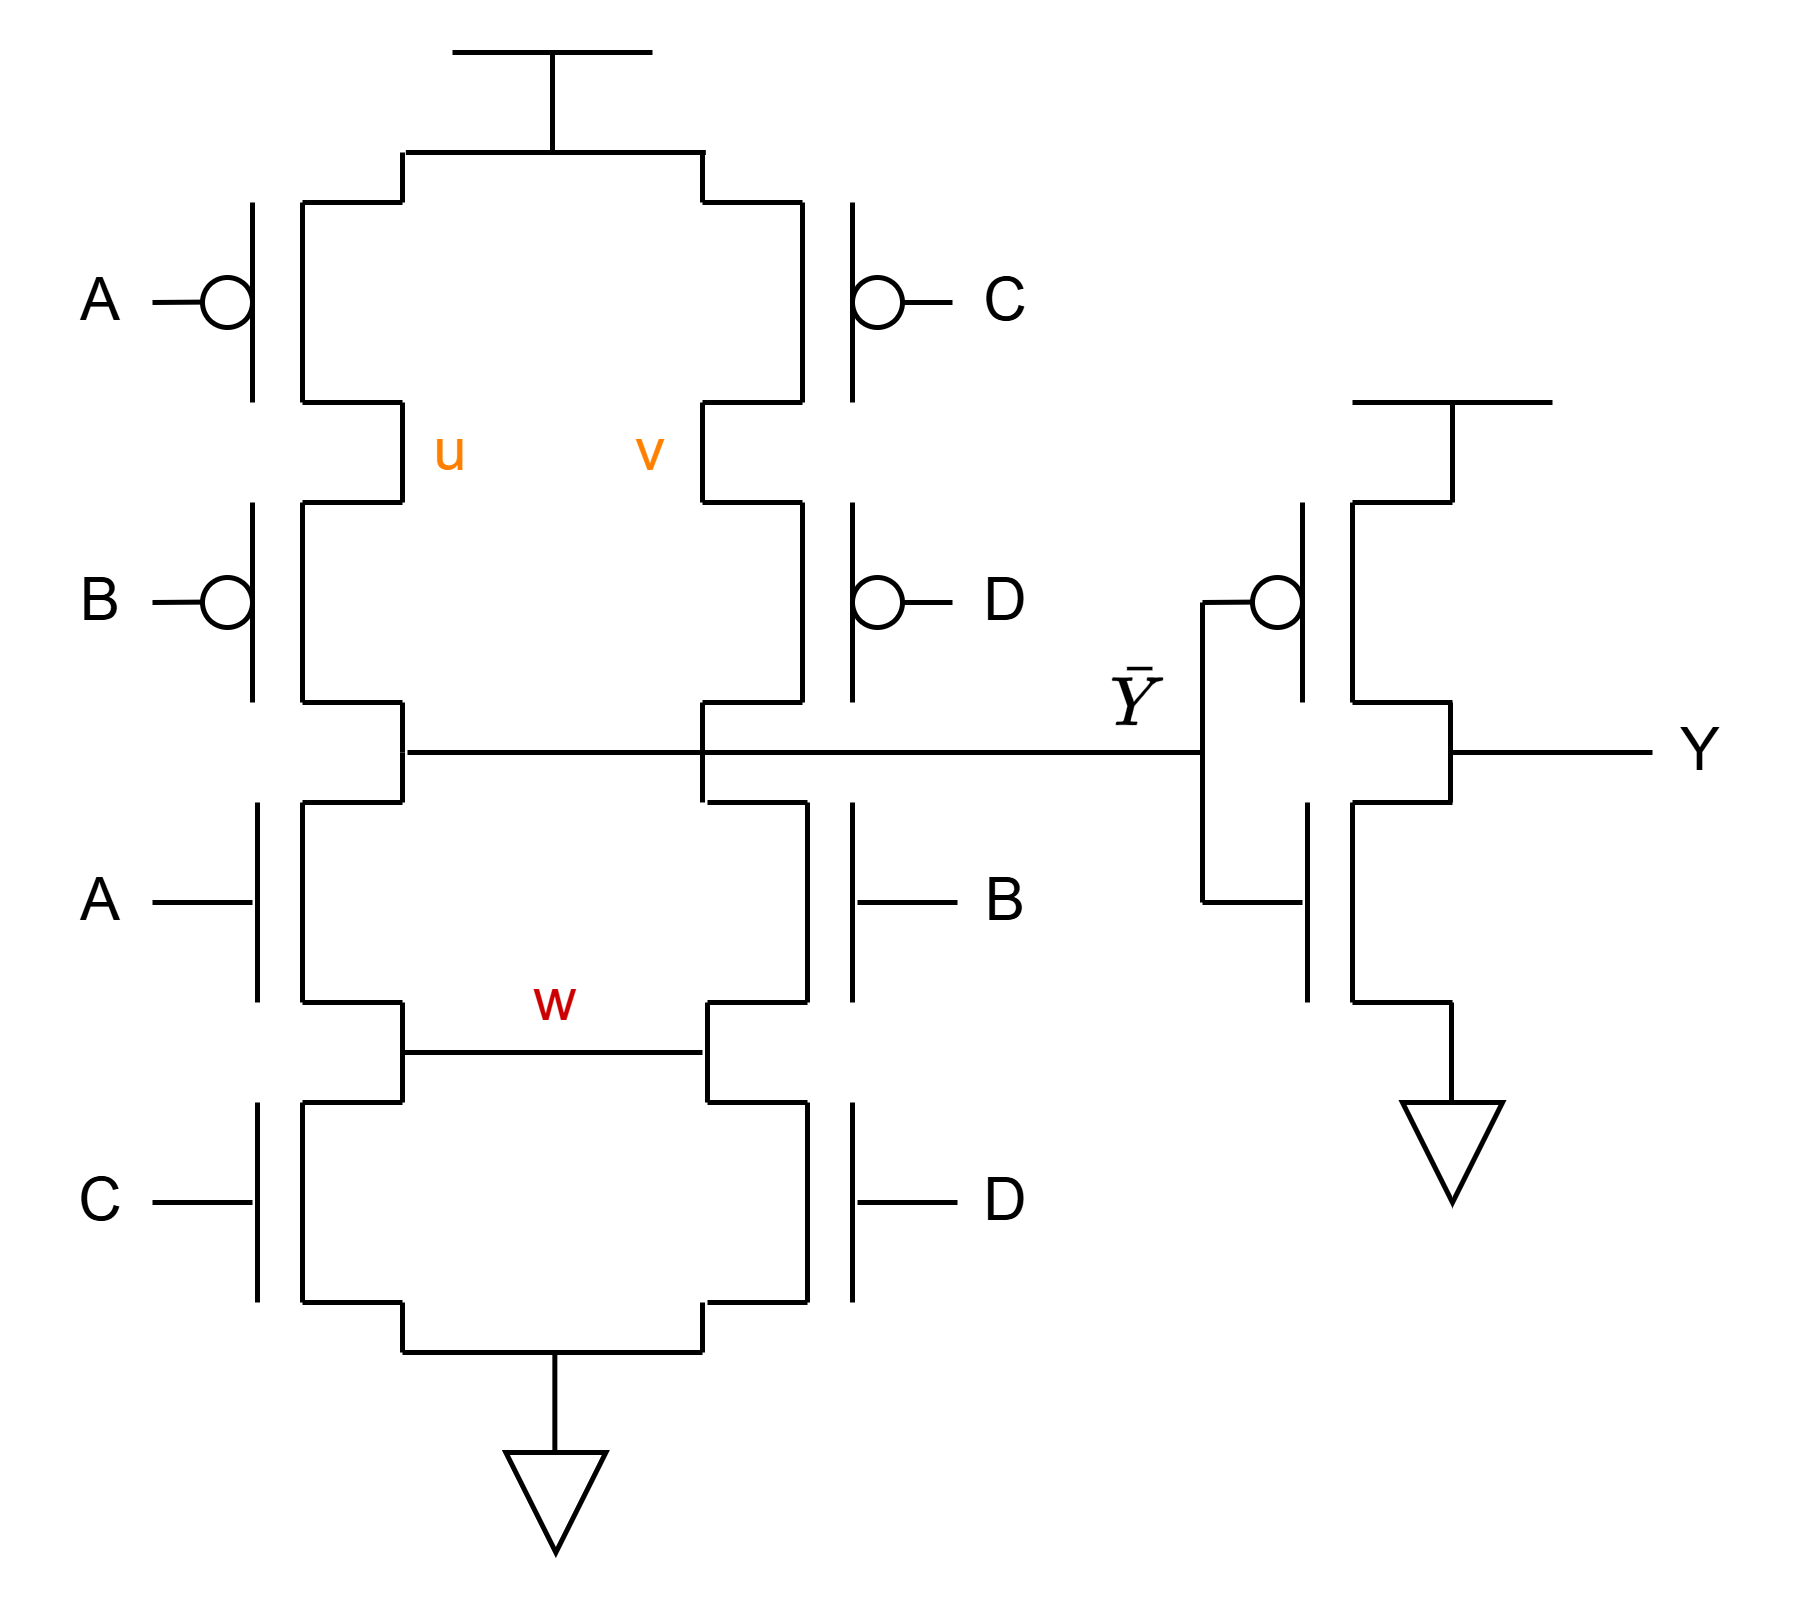
\includegraphics[width=0.5\textwidth]{cmos_layout_problem_2a.png}}}
				\caption{CMOS Layout for Problem 2a}
				\label{fig::cmos_layout_problem_2a}
			\end{figure}
			
			To determine the order of the stick diagram inputs, we must find a Euler Path through the circuit. The Euler Path for this circuit has been traced out in the logic diagram shown in Figure \ref{fig::logic_diagram_problem_2a}.
			
			\begin{figure}[H]
				\centerline{\fbox{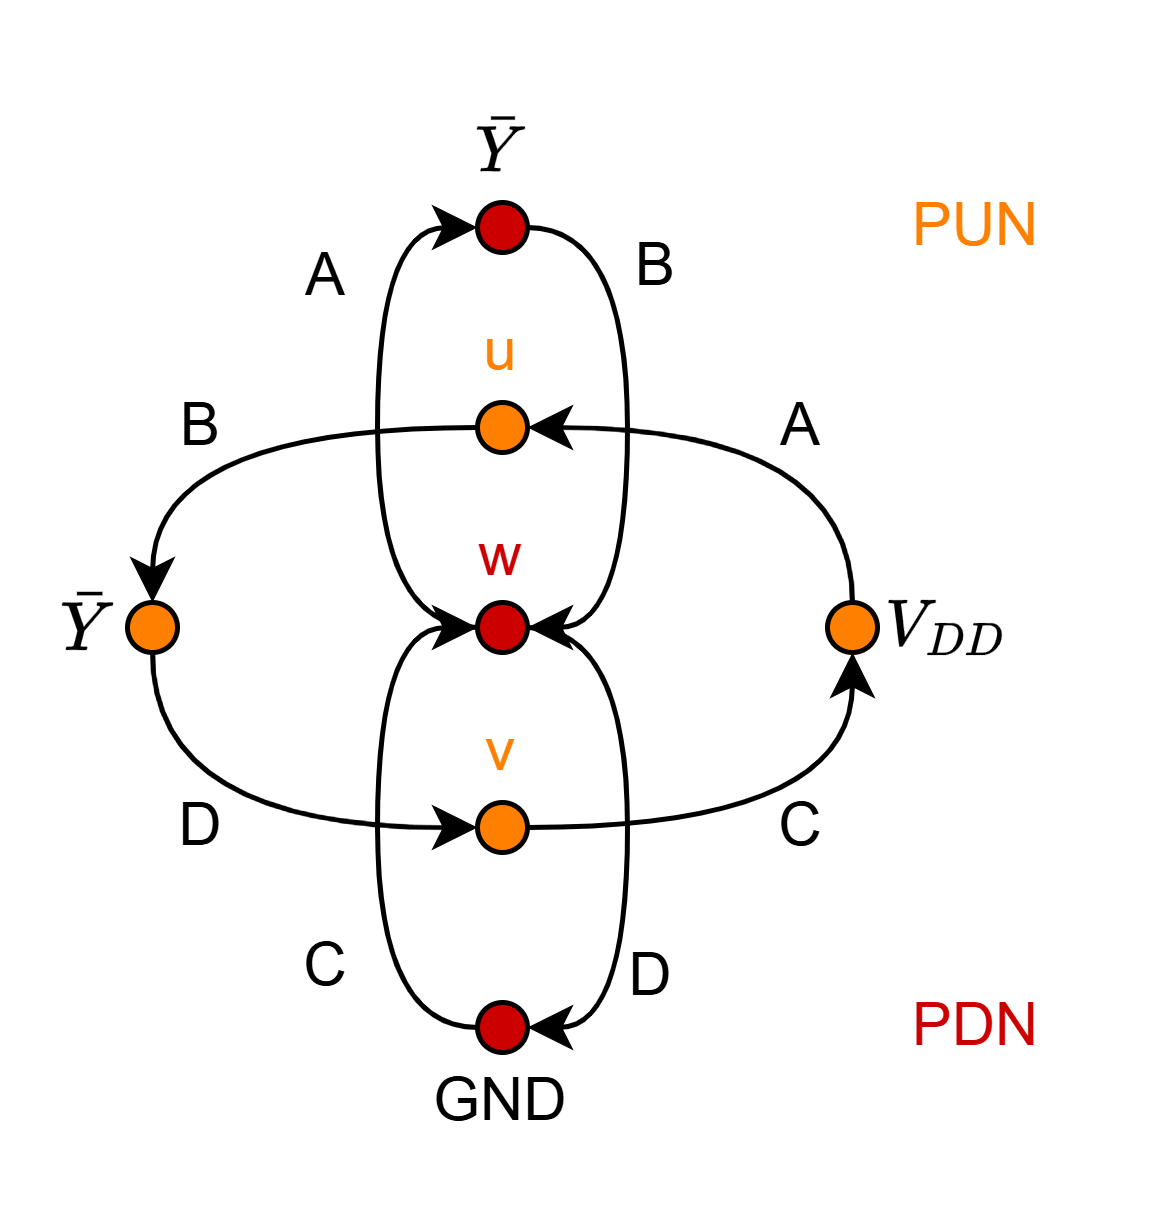
\includegraphics[width=0.4\textwidth]{logic_diagram_problem_2a.png}}}
				\caption{Logic Diagram for Problem 2a Illustrating Euler Path}
				\label{fig::logic_diagram_problem_2a}
			\end{figure}
			
			The Euler path can be found by independently tracing through all the nodes of the pull-down and pull-up networks once and only once. The path we find must also be consistent between the pull-up and pull-down networks. For this example, we determine the following input ordering: A, B, D, and C. This ordering we find using the Euler path helps us generate a layout without diffusion breaks. Using the requested input ordering, we come up with the stick diagram shown in Figure \ref{fig::stick_diagram_problem_2a}. Note that we have also added an inverter to get $Y$ instead of $\bar{Y}$
			
			\begin{figure}[H]
				\centerline{\fbox{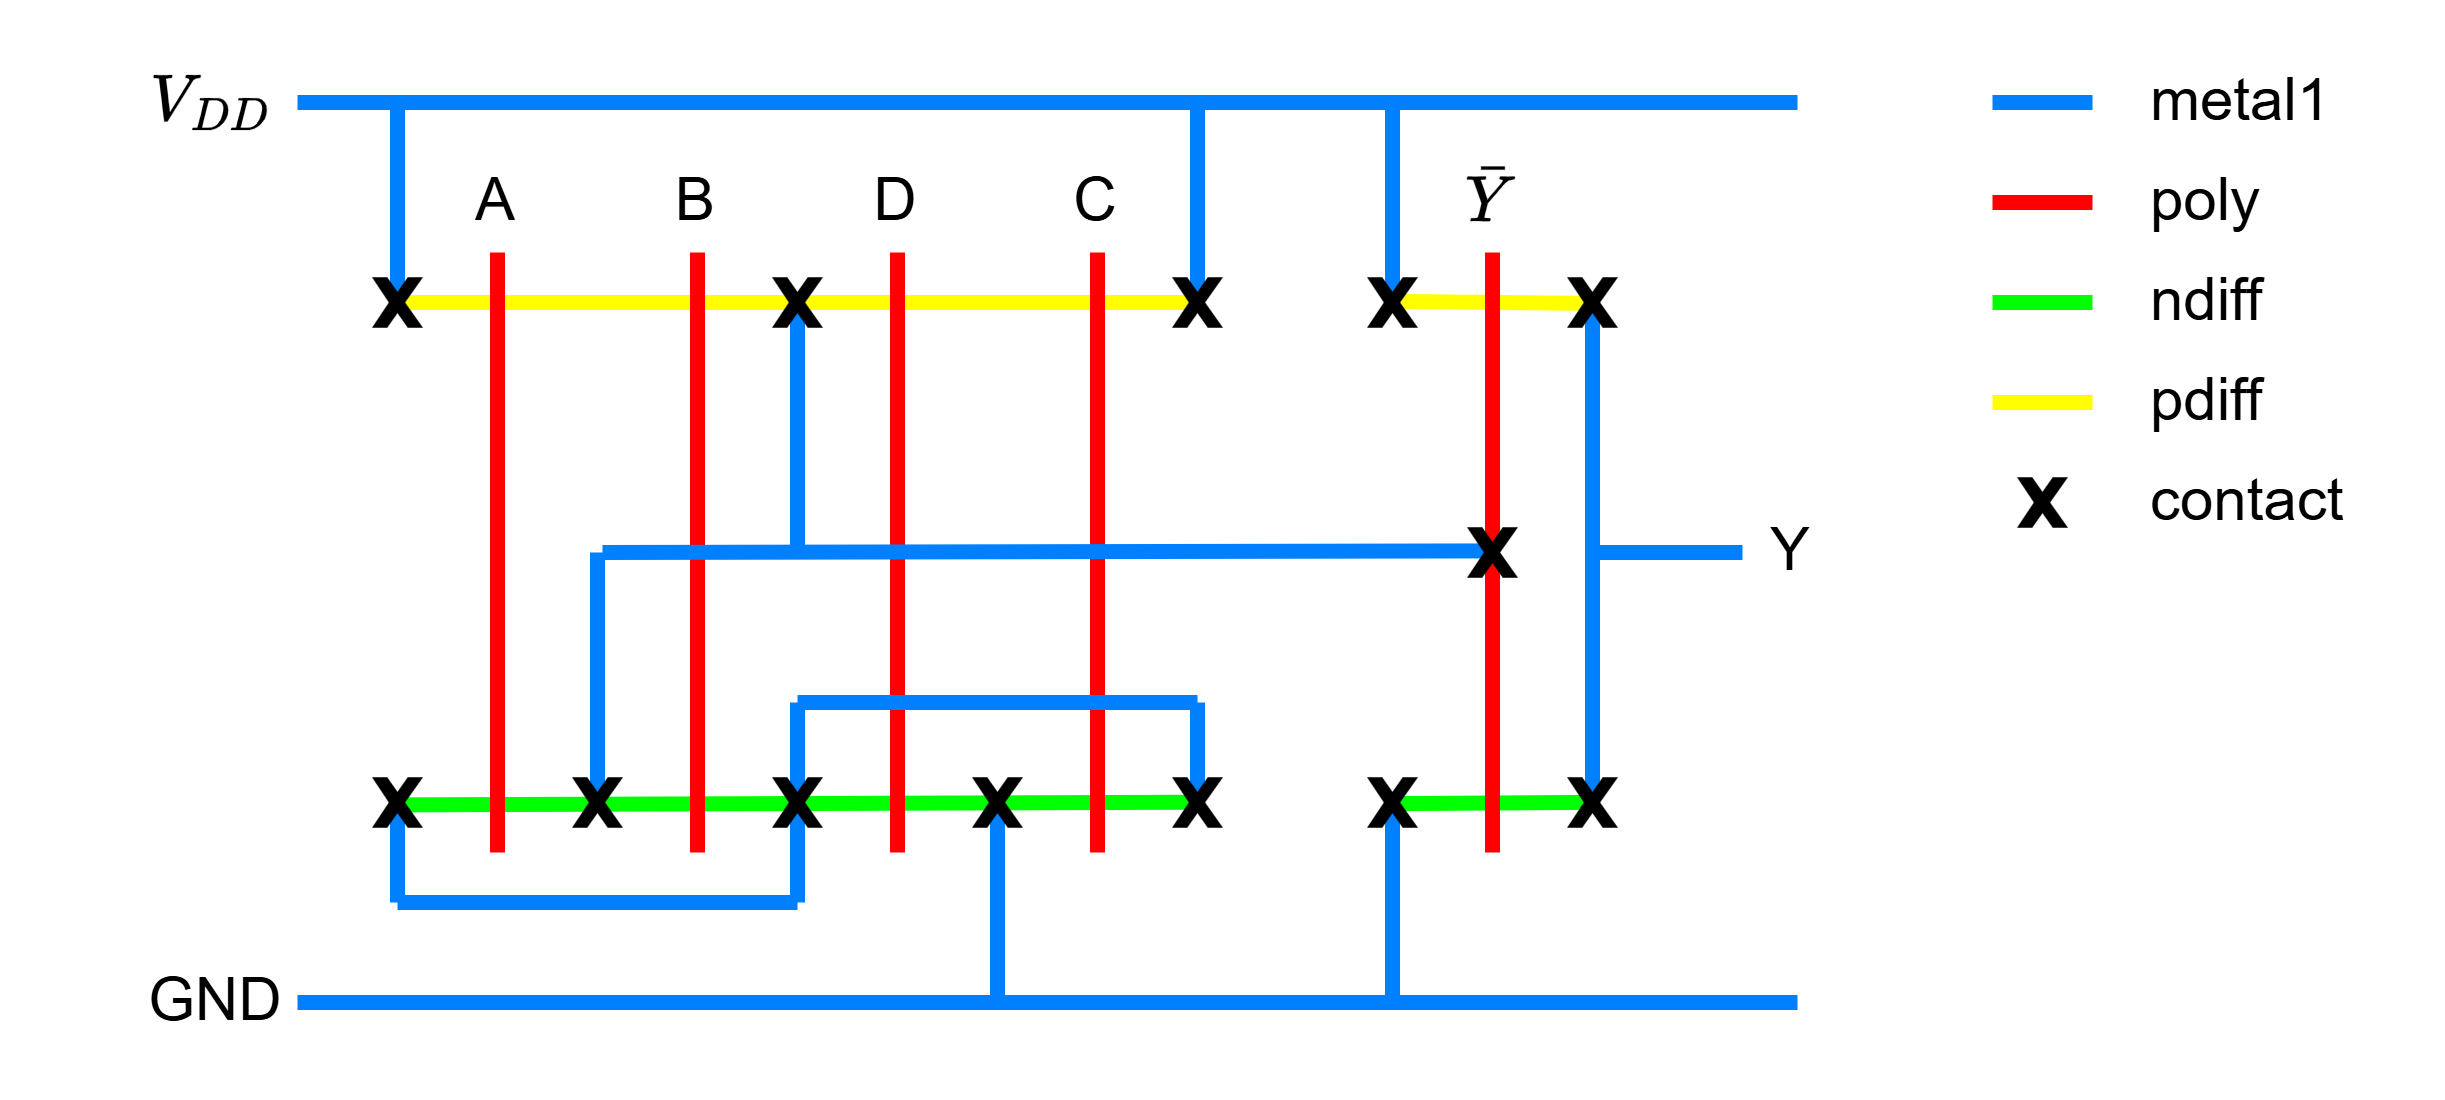
\includegraphics[width=0.6\textwidth]{stick_diagram_problem_2a.png}}}
				\caption{Stick Diagram for Problem 2a}
				\label{fig::stick_diagram_problem_2a}
			\end{figure}
			
			\item $Y = \overline{A \cdot B + C \cdot D}$
			
			The provided boolean expression is now in complemented form, so no inverter is needed. Following the steps in part a), we design the pull-down circuit for this part of the problem. The resulting pull-down circuit is shown in the bottom half of Figure \ref{fig::cmos_layout_problem_2b}. Using the rule of conduction complements, we then design the required pull-up circuit, which is shown in the top half of Figure \ref{fig::cmos_layout_problem_2b}.
			
			\begin{figure}[H]
				\centerline{\fbox{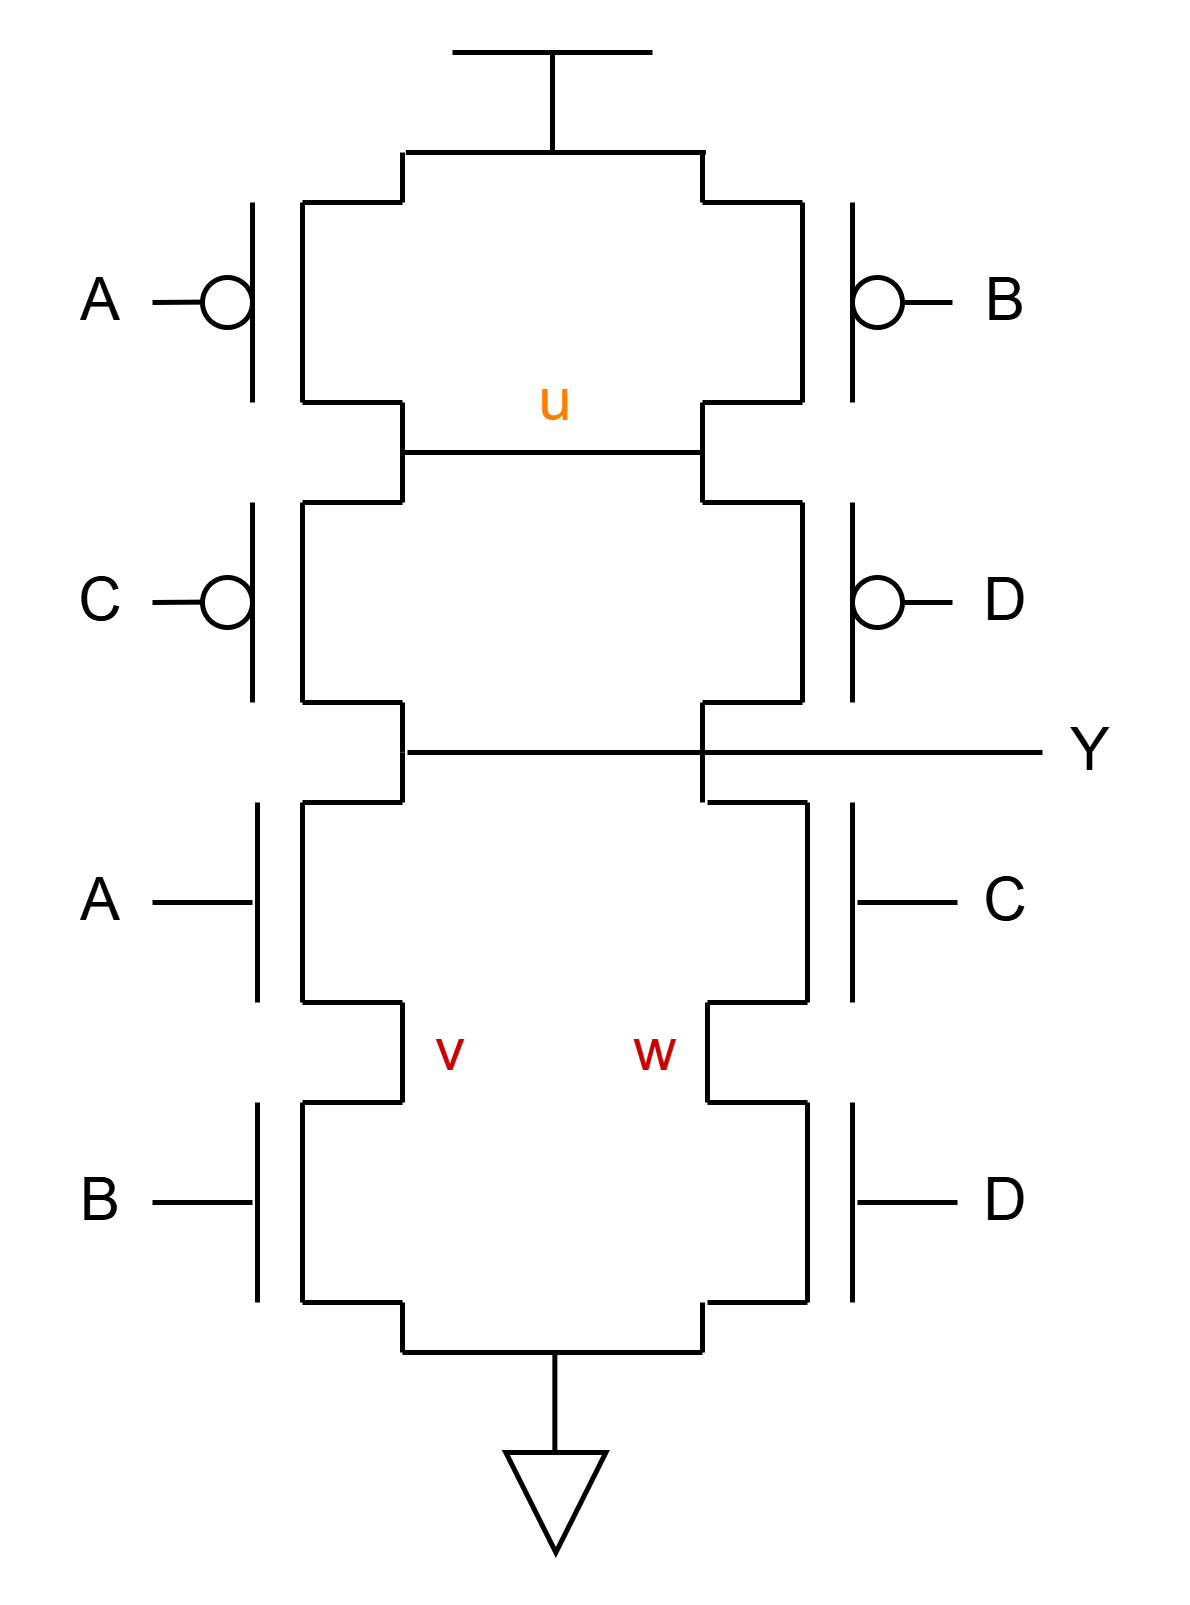
\includegraphics[width=0.35\textwidth]{cmos_layout_problem_2b.png}}}
				\caption{CMOS Layout for Problem 2b}
				\label{fig::cmos_layout_problem_2b}
			\end{figure}
			
			Next, we determine the ordering of the stick diagram inputs by find the Euler Path through the circuit. This path is illustrate in the logic diagram shown in Figure \ref{fig::logic_diagram_problem_2b}. Using the logic diagram, we find an input ordering of A, B, D, and C, identical to what was found in part a).
			
			\begin{figure}[H]
				\centerline{\fbox{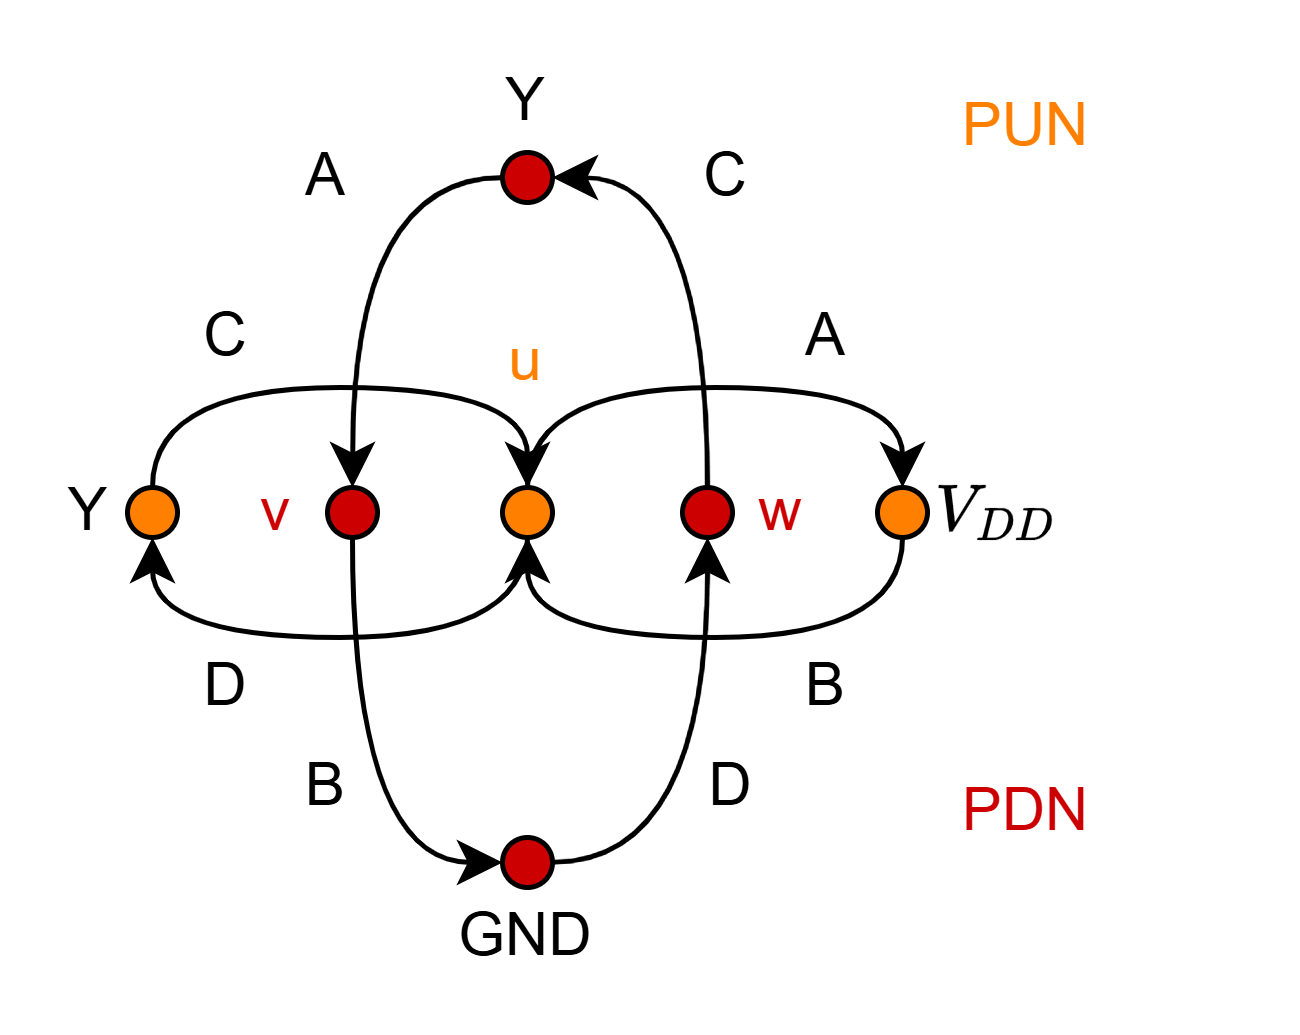
\includegraphics[width=0.45\textwidth]{logic_diagram_problem_2b.png}}}
				\caption{Logic Diagram for Problem 2b Illustrating Euler Path}
				\label{fig::logic_diagram_problem_2b}
			\end{figure}
			
			Finally, with the order of inputs, we can create the stick diagram shown in Figure \ref{fig::stick_diagram_problem_2b}.
			
			\begin{figure}[H]
				\centerline{\fbox{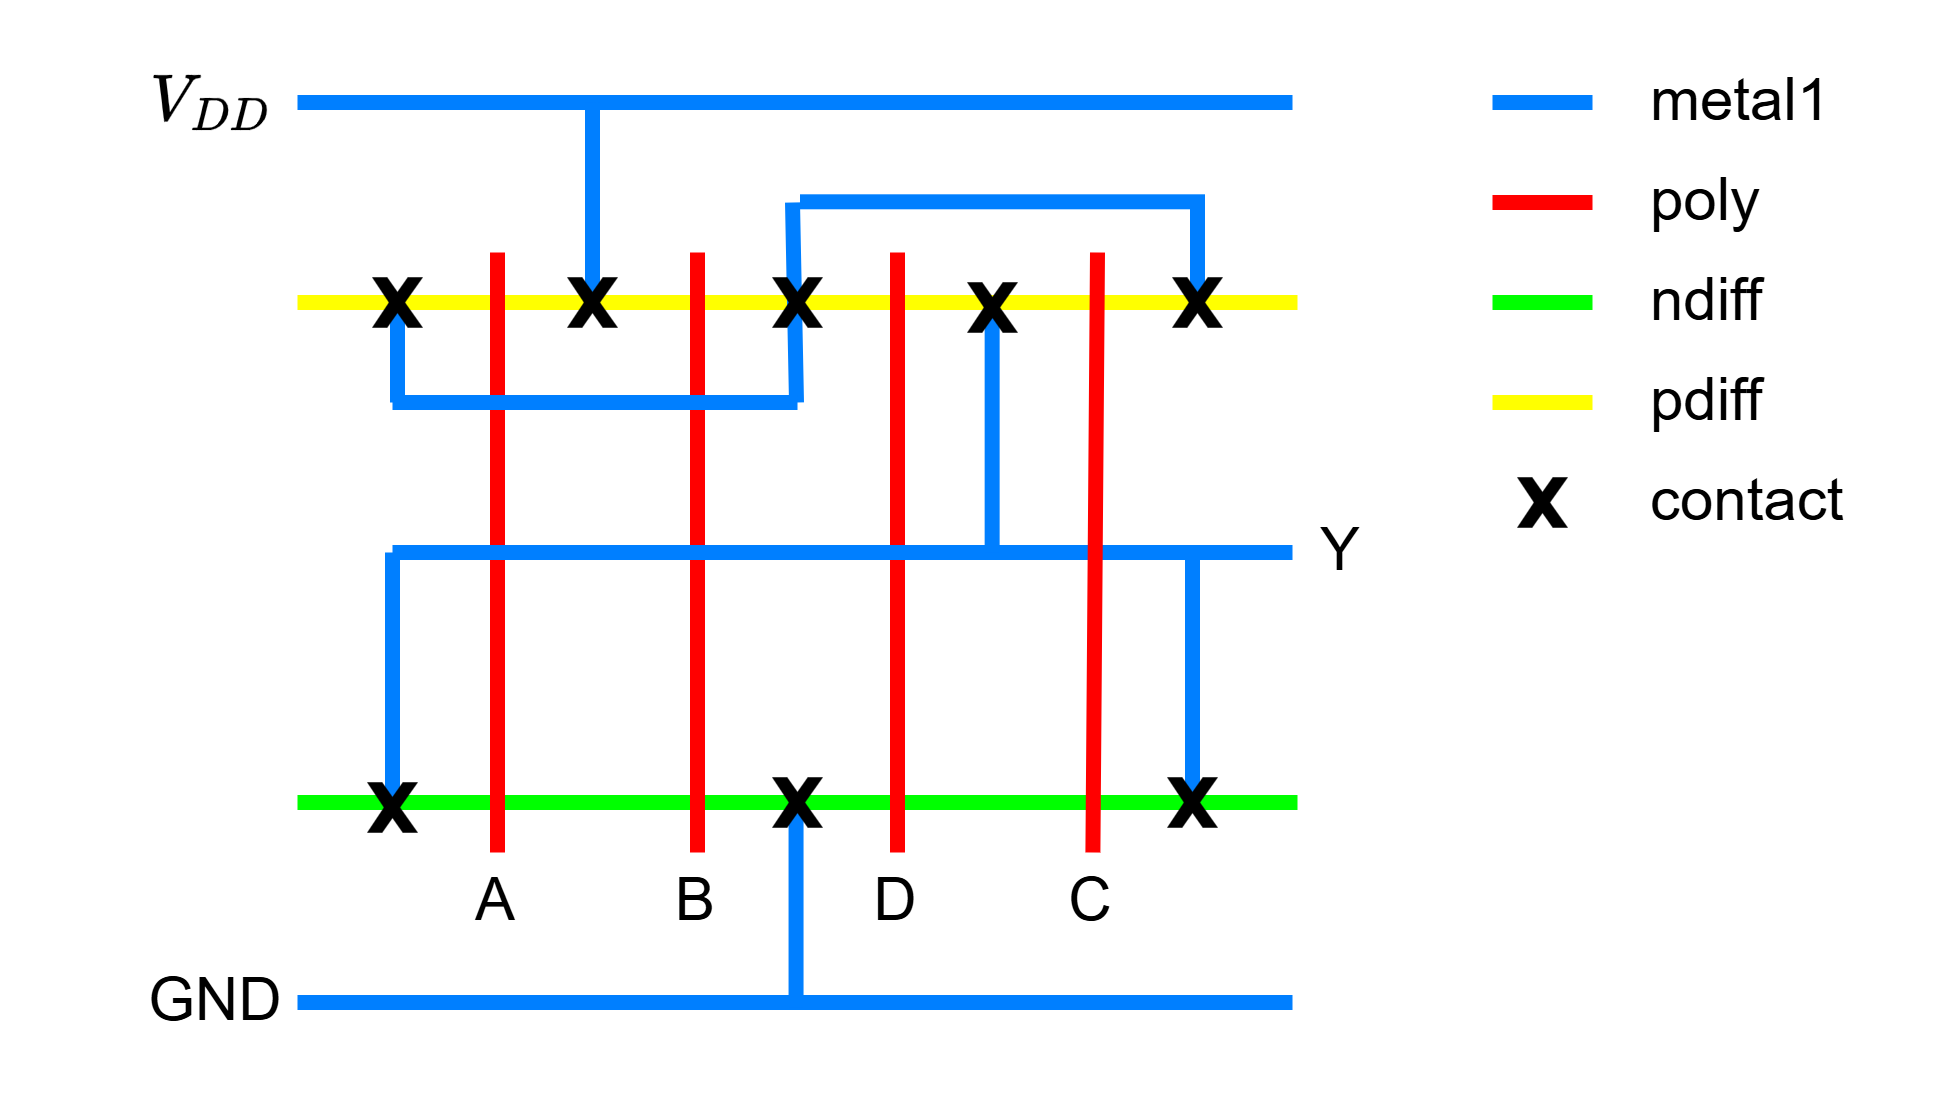
\includegraphics[width=0.5\textwidth]{stick_diagram_problem_2b.png}}}
				\caption{Stick Diagram for Problem 2b}
				\label{fig::stick_diagram_problem_2b}
			\end{figure}
		\end{enumerate}
		
		\item Using the Stick diagrams designed in the previous, question, Calculate the Area Estimation in terms of $\lambda$.
			
		We can estimate the area of the fabricated design by counting wiring tracks. Each wire track has a pitch of $8\lambda$. If we count the number of wires parallel to $V_{DD}$ (including $V_{DD}$), we can estimate the height of the cell. Similarly, we can estimate the width of the cell by counting the number of wires parallel to the polysilicon gates.
		
		For the layout in part a), we can view the circuit as two standard cells (one which produces $\bar{Y}$ and another which inverts it). The first cell is 7 wires tall and 5 wires wide ($56 \lambda \times 40 \lambda$), and the second cell is 4 wires tall and 2 wires wide ($32 \lambda \times 16 \lambda$). However, all our standard cells must have the same height and can only vary in width. Therefore, we must increase the size of the inverter to $56 \lambda \times 16 \lambda$. This results in a total area of $56 \lambda \times 56 \lambda$.
		
		The area of the layout in part b) is more straightforward to compute than the layout in part a). It is 7 wires tall and 5 wires wide, which results in an area of $56 \lambda \times 40 \lambda$.
		 
	\end{enumerate}
	
	\pagebreak
	\appendix
	\section{Verilog Ripple Carry Adder Written with Primis AI}
	\label{appendix::ripple_carry_adder}
	\lstset{style={verilog-style}}
	\lstinputlisting{ripple_carry_adder.v}
	
	\pagebreak
	\section{Verilog Testbench Written with Primis AI}
	\label{appendix::testbench}
	\lstset{style={verilog-style},showstringspaces=false}
	\lstinputlisting{ripple_carry_adder_tb.v}
\end{document}